%\renewcommand\labelitemi{\textcolor{blue}{$\bullet$}}  
\renewcommand\labelitemi{\textcolor{blue}{$\bullet$}}  
\renewcommand\normalcolor{\color{blue}}  %for titles, etc.
\renewcommand\Black{\color{black}}        %for headers, etc.
\renewcommand\labelitemii{\textcolor{DarkGreen}{$\star$}}  
\color{black}                             %for normal text

%\renewcommand\normalcolor{\color{yellow}}  %for titles, etc.
%\renewcommand\Black{\color{white}}        %for headers, etc.
%\color{white}                             %for normal text


\foilhead{\textcolor{red}{E} Dynamics of the ISM}
\leftheader{E: ISM dynamics }
\vpagecolor[blue]{RGBblack}                 %blue to black vertical gradient
\LogoOff
\bgclear

\begin{enumerate}
\item J shocks \label{item:Jshocks}
\item C shocks \label{item:Cshocks}
\item Supernova remnants \label{item:SNRs}
\item Ionisation fronts \label{item:HIIs}
\item Cloud equilibrium \label{item:eq}
\end{enumerate} 


\renewcommand\labelitemi{\textcolor{blue}{$\bullet$}}  
\renewcommand\normalcolor{\color{blue}}  %for titles, etc.

\foilhead{\textcolor{red}{E-\ref{item:Jshocks}} J shocks}
\leftheader{E-\ref{item:Jshocks} J shocks}

\renewcommand\labelitemi{\textcolor{blue}{$\bullet$}}  
\renewcommand\Black{\color{black}}        %for headers, etc.
\renewcommand\labelitemii{\textcolor{DarkGreen}{$\star$}}  
\color{black}                             %for normal text

\LogoOff
\bgclear
\pagecolor{white}

\begin{itemize}

\item References: 

Tielens 2005\\ Draine \& Mc~Kee, 2003, ARA\&A, 31, 373 \\


\item Shocks are irreversible processes: ordered kinetic energy from
  stellar winds, supernova shock waves, etc ..., is converted into
  heat and chemical processes, with a concomitant entropy increase.

\item Shocks are at the origin of the large-scale structure of the ISM
  and of the hot-shocked plasma phase ($\sim 10^{6}$~K). 

\item There are two broad types of shocks: J (jump) shocks and C
(continuous) shocks. J-types are strong shocks that occur in all
phases of the ISM, while C shocks are found in (magnetised) molecular
clouds. The main difference between C and J shocks is the shock
velocity. The minimum velocity for J-shocks is $\sim$40~km~s$^{-1}$.

\end{itemize}

\foilhead{\textcolor{red}{E-\ref{item:Jshocks}} J shocks}


\begin{itemize}

\item In shocks the preferred reference system is that of the shock
  itself: the preshock gas flows towards the shock at the shock
  velocity $v_s$, while the postshock gas moves with the shock front,
  so has $\sim 0$ velocity relative to the shock. 


\end{itemize}

\begin{center}
  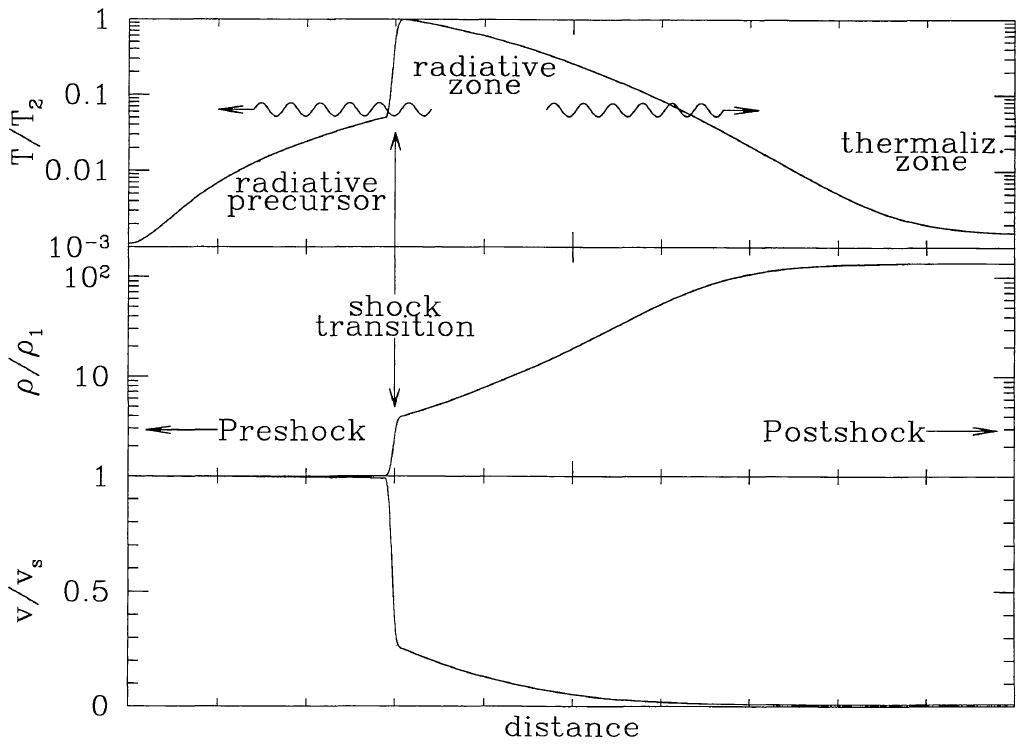
\includegraphics[width=14cm,height=!]{./E/fig_Jshocks.jpg}
\end{center}

\foilhead{\textcolor{red}{E-\ref{item:Jshocks}} Jump conditions}

\begin{itemize}

\item J shocks are supersonic discontinuities. The speed of the shock
  can be expressed with the Mach number, $M = v_s/c_s$, where $c_s =
  \sqrt{\partial p / \partial \rho |_S }$ is the sound speed. For an
  adiabat $P \propto \rho^\gamma$ and the equation of state $P = \rho
  k T / \mu$, with $\gamma = 5/3$, $c_s = \sqrt{5/3 k T / \mu}$.

\item The fluid equations of motions take on simple forms when
  integrated across sharp discontinuities. These are the
  Rankine-Hugoniot jump conditons, which express the conservation of
  mass, momentum and energy flux.

\item The flux of any scalar quantity per unit mass $\phi$ is $\phi
  \rho v$. Examples: 
\begin{itemize}
\item mass flux is $\rho v$, 
\item momentum flux is $(\rho v)
  v$ ($v$ is the momentum per unit mass), 
\item kinetic energy flux is  $(\rho v) (v^2 / 2)$,
\item internal energy flux  $(\rho v) (u / \rho)$, where $u = \sum_i
  (u_i + n_i I_i)$ is the internal energy per unit volume, and $I_i$ is
  the binding energy of specie $i$, with number density $n_i$. 

\end{itemize}
\end{itemize}

\foilhead{\textcolor{red}{E-\ref{item:Jshocks}} Rankine-Hugoniot
  conditions}

\begin{eqnarray}
\rho_0 v_0  & =  & \rho_1 v_1, ~~~ \text{mass} , \\
\rho_0 v_0^2 + P_0   & =  & \rho_1 v_1^2 + P_1, ~~~ \text{momentum} , \\
\frac{1}{2} v_0^2 + \frac{u_0}{\rho_0} + \frac{P_0}{\rho_0}   & =  & 
\frac{1}{2} v_1^2 + \frac{u_1}{\rho_1} + \frac{P_1}{\rho_1}
, ~~~ \text{energy}. \label{eq:energy}
\end{eqnarray}

Eq.~\ref{eq:energy} derives from equating $P_0 v_0 - P_1 v_1 $, the
work done by the shock per unit time, to the net energy flux through
the shock: $E_1 - E_0$, where \[ E_i = \rho_i v_i \left(\frac{1}{2}
v_i^2 + \frac{u_i}{\rho_i}\right) . \] Note Eq.~\ref{eq:energy}
expresses energy conservation for an adiabatic shock - without
radiative losses, which are important for the evolution of the shock.


\foilhead{\textcolor{red}{E-\ref{item:Jshocks}} Solution of the jump
  conditions} 

For an ideal gas in an adiabatic shock, manipulation of the jump
conditions gives ({\color{red} tarea}):
\begin{eqnarray}
\frac{P_1}{P_0} & = & \frac{2\gamma M^2}{\gamma + 1} - \frac{\gamma -
  1}{\gamma +1}, \\
\frac{\rho_0}{\rho_1} & = & \frac{\gamma -
  1}{\gamma +1} + \frac{2}{\gamma + 1} \frac{1}{M^2}, \label{eq:dens} \\ 
v_i^2  & = & \frac{1}{\rho_i^2} (P_1 - P_0) \left(\frac{1}{\rho_0} - \frac{1}{\rho_1}\right)^{-1}.  
\end{eqnarray}
For strong shocks, $M \gg 1$, 
\begin{eqnarray}
\frac{\rho_1}{\rho_0} & = & \frac{\gamma + 1 }{\gamma -1 } ~~(~= 4~~
\text{for an ideal monatomic gas}), \label{eq:Jshock1} \\
P_1 & = & \frac{2}{\gamma + 1} \rho_0 v_0^2 ~~~( = \frac{3}{4} \rho_0
v_0^2), \label{eq:pres1}\\ 
v_1 & = & v_0 /4. \label{eq:Jshock2}
\end{eqnarray}

\foilhead{\textcolor{red}{E-\ref{item:Jshocks}} Temperature rise at
  the shock front} 

For an ideal gas, Eq.~\ref{eq:pres1} gives 
\[T_1 = \frac{2 (\gamma - 1)
}{\gamma + 1} \frac{\mu v_0^2}{k} = \frac{3}{16} \frac{\mu}{k}
v_0^2,~~~{\text{for a monatomic gas}}.\] 


In a cosmic mix with a He abundance of -1~dex, $\mu / m_p = \sum n_i
m_i / \sum n_i \approx 0.56$ for fully ionised gas , $\approx 1.3$ for
neutral gas, and $\approx 2.4$ for molecular gas.


 Thus, independently
of the preshock phase,
\[ T_1 \approx \frac{\mu}{m_p} 2.5~10^{5} \left(
\frac{v_0}{100~\mathrm{km~s}^{-1}} \right)^2 \text{~K} \]


\foilhead{\textcolor{red}{E-\ref{item:Jshocks}} Downstream
conditions} 

Away from the (idealised) adiabatic shock front and into the postshock
region, radiative losses decrease the temperature. 

The flux of radiative energy $F_\mathrm{rad}$ varies as
\[ \frac{d}{dz}F_\mathrm{rad} = n^2\Lambda  - n \Gamma  - 4 \pi \kappa
J, \]
where $z$ is a coordinate along the shock propagation, $n$ is number
density, $\Lambda$ and $\Gamma$ are the cooling and heating rates,
respectively, and $J$ is the average intensity from other regions in
the shock. 

At some distance from the shock front, in a region which we may label
as ``$2$'', the shocked gas will eventually relax to its preshock
conditions, in region ``0''. We may apply the jump conditions to the
0--2 discontinuity, with an isothermal gas ($\gamma = 1$), so that
Eq.~\ref{eq:dens} gives \[ \rho_2 / \rho_1 = M^2.\] We see shock waves
are very compressive!


\foilhead{\textcolor{red}{E-\ref{item:Jshocks}} Downstream
conditions} 

However, at very high temperatures the cooling rate is dominated by
recombinations, with a rate $\Lambda \propto \sqrt{T}$, so that the
cooling time scale, $\tau_\mathrm{cool} = k T / (n \Lambda(T)) \propto
\sqrt{T}$. 

Hence, if the shock is very strong $M\gg1$, the postshock temperature
can be arbitrarily high, and $\tau_{cool}$ correspondingly long - and
possibly even longer than the lifetime of the shock (or the dynamical
time scale). If so then the postshock region never relaxes, as is the
case of the ISM hot-shocked by SNRs. 

\foilhead{\textcolor{red}{E-\ref{item:Jshocks}} Precursor ionisation} 

In fast shock, if the postshock temperature reaches $\sim 10^5~$K,
then H~{\sc\,i} is collisionally ionised and radiates in the Lyman
continuum. The correspond ionising radiation overtakes the shock front
and ionises the preshock gas. 


\begin{center}
  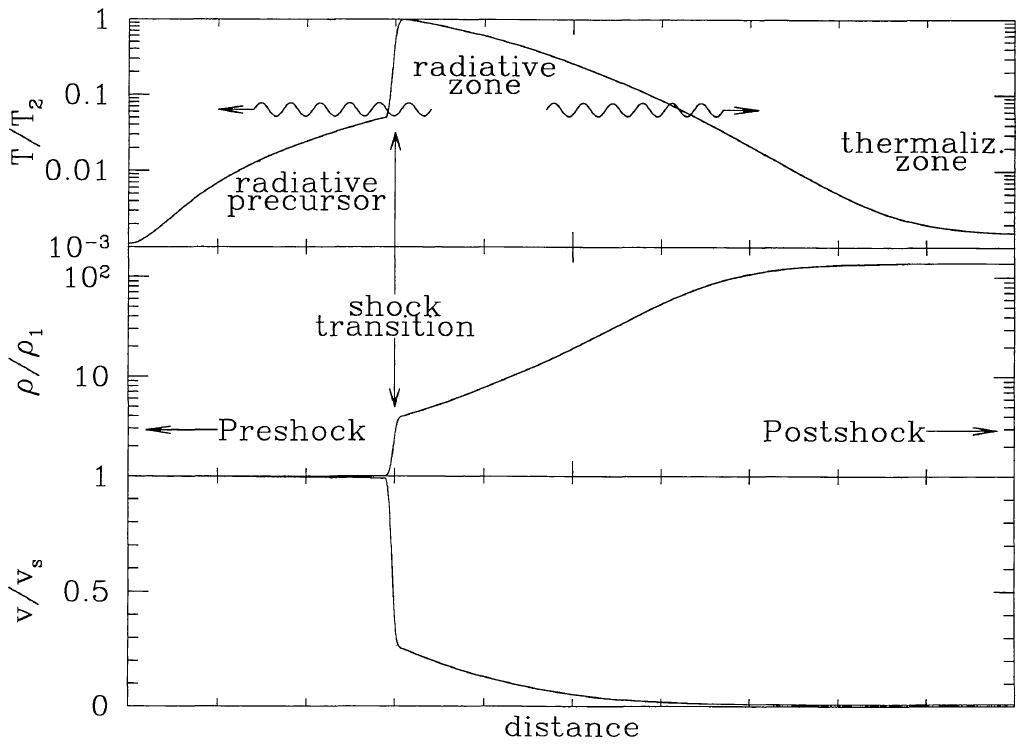
\includegraphics[width=14cm,height=!]{./E/fig_Jshocks.jpg}
\end{center}




\foilhead{\textcolor{red}{E-\ref{item:Jshocks}} J shock chemistry} 

\begin{itemize}
\item Shocks lead to dissociation/ionisation and eventually to
  molecule formation in the relaxation zone behind the shock front. 

\item  The shock chemistry is radically different from the
  ion-molecule chemistry that occurs in quiescent dark clouds. 

\item Collisional H$_2$ dissociation occurs for gas at $>10^5~$K, or
  shock velocities higher than 50~km~s$^{-1}$. 

\item In the postshock region, with elevated temperatures, the
  chemistry taps on the gas internal energy to generate molecules via
  endothermic reactions.  The key players in this chemistry are H,
  H$_2$ and O (assuming a cosmic mix with O$>$C). 

  \begin{itemize}
    \item If H$_2$ is not dissociated, then reactions with O leads to
      the formation of H$_2$O, so that the most abundant molecules are
      H$_2$, H$_2$O, CO, and O$_2$. Important trace molecules,
      characteristic of non-dissociating shocks, are CH$^+$, SiO,
      H$_2$S. 

      \item If H$_2$ is dissociated, loose H atoms collisionally
        dissociate molecules so that most of the gas is atomic (as
        expected from $\sim$~1000~K gas). 
\end{itemize}
\end{itemize}

\foilhead{\textcolor{red}{E-\ref{item:Jshocks}} J shock spectra} 

\begin{itemize}

\item The spectra of non-ionising shocks reflect their chemistry. 

\item Ionising shocks lead to very hot, 10$^6$~K, gas and bright in
  X-rays. If the density is low, then the cooling timescale exceeds
  the shock lifetime, and columns are low, so that not much emission
  is found at UV-optical-IR wavelengths.

\item If driven into dense media, ionising shocks may relax in the
  post-shock region, which is very compressed. The columns are then
  high enough for the detection of britght optical/IR collisionally
  excited fine structure lines.  


\newpage
\item Since the relaxation zones dominate by mass the fully-ionised
  regions, the spectra of ionising shocks is dominated by
  low-excitation species, which are normally found in
  higher-ionisation stages in H\,{\sc ii} regions. 

\item Two (among many) popular diagnostics for shock excitation
  versus photionisation are:

\begin{itemize}
\item The ratio of [N\,{\sc ii}]~$\lambda\lambda$6548,6584 to
  H$\alpha$ $\lambda$6565 - [N\,{\sc ii}] is not as bright in H\,{\sc
    ii} regions than in shocks  
 
\item The ratio [Fe\,{\sc ii}]~1.644$\mu$m / Br$\gamma$~2.166$\mu$m is high in
  shocks, because in H\,{\sc ii} regions Fe would be found in higher
  ionisation stages.


\end{itemize}

\end{itemize}

\foilhead{\textcolor{red}{E-\ref{item:Cshocks}} C shocks} 

\begin{itemize}

\item For interstellar conditions, the magnetic field is ``frozen'' to
  matter.  The magnetic flux $\Phi = \int_S \vec{B}.\vec{dS}$, where
  $S$ is some surface tied to the fluid, is constant.

\item When the gas is compressed perpendicular to $\vec{B}$, the field
  intensity increases so that $ \Phi = S B$ is kept constant. As a
  result \begin{equation} B \approx
    \sqrt{n/1~\mathrm{cm}^{-3}}~\mu\mathrm{G} .\label{eq:Bscale} \end{equation}

\item Thus magnetic field intensities in dense molecular gas are high,
  and we must modify the shock equations to include the coupling of
  the magnetic field to the residual ionisation induced by cosmic ray
  ionizations. 

\end{itemize}


\foilhead{\textcolor{red}{E-\ref{item:Cshocks}} C shocks} 


\begin{itemize}

\item Cosmic ray ionisation predicts an ionisation fraction of $x
  \approx 10^{-8}- 10^{-7}$, as observed (e.g. Wootten et al., 1979,
  ApJ, 234, 876).

\item Most of the negative charge in molecular gas is found in PAH
  anions - they sweep out all the $e^-$ ejected by the cosmic ray
  ionisation of H$_2$. 

\item Magnetised shocks are thus 2 fluid shocks: the ions, which
  directly couple to the magnetic field, and the neutrals, which lag
  behind the ions and are coupled to the field by collision and
  frictional drag with the ions.

\end{itemize}

\leftheader{E-\ref{item:Cshocks} C shocks}

\foilhead{\textcolor{red}{E-\ref{item:Cshocks}} C shocks} 

\begin{itemize}

\item The linearisation of the hydromagnetic equations shows that
  magnetised media sustain a wide variety of magnetosonic waves (an
  extension of sound waves).

\item The type of Alfv\'en waves that is most relevant to shocks are
  transversal oscilations of the magnetic field lines, as in vibrating
  strings. Their speed is $v_A = B (4 \pi \rho_i)^{-1/2}$, where
  $\rho_i$ is the mass density of the ion fluid. 

\item The Alv\'en waves propagate the shock signal upstream,
  compressing the ions and dragging the neutrals. The wave energy is
  dissipated by ion-neutral friction, which raises the temperature. 

\item The shock front is merged with the relaxation layers. Thus
  magnetic shocks are continuous (C-shocks).

\end{itemize}


\foilhead{\textcolor{red}{E-\ref{item:Cshocks}} Structure of C shock:
  shock width} 

\begin{itemize}

\item The characteristic length over which the neutral fluid velocity
  changes is $L \approx v_d / (n_i k_L)$, where $v_d = v_i - v_n$ is
  the ion-neutral drift velocity (which can be of the order of the
  shock velocity since the ions are first set in motion, and
  subsequently drag the neutrals - $v_d$ values can be as high as
  $\sim$30~km~s$^{-1}$), and $k_L = \langle w \sigma_{in} \rangle
  \approx 10{-7}$cm$^{3}$~s$^{-1}$ is the Langevin rate (the number of
  ion-neutral collisions per ion per unit time, where $w$ is
  ion-neutral relative velocities in the frame of the neutrals).

\item As for the calculation in J-shocks, the maximum compression of
  ions is $(n_i / n_{i,0}) \approx v_s / v_A $, where $v_s/v_A$ is
  an extension of the Mach number and $n_{i,0}$ is the pre-shock ion
  density. A working number for the ion-neutral drift velocity is half
  the shock velocity.  Thus 
\[ L \approx \frac{v_A }{2 n_{i,0} k_L} .\]

\item Assuming Eq.~\ref{eq:Bscale}, we obtain $L \approx 1.1~10^5 /
  (n_{i,0} k_L) \approx 10^{15}~$cm if the pre-shock proton density is
  $10^5$ and the ionisation fraction is $x \sim 10^{-8}$. 


\end{itemize}


\foilhead{\textcolor{red}{E-\ref{item:Cshocks}} Structure of C shock:
  thermal balance}



\begin{itemize}

\item Heating comes from the mechanical energy of the shock wave,
  hence

\[ n \Gamma \approx  \underbrace{\rho_0 v_s^2}_{\text{shock kinetic energy
  density}} \overbrace{(v_s / L)}^{\text{shock timescale}} . \]

\item Shock cooling comes from H$_2$ rotational lines:
$ n^2 \Lambda(T) = 2.5~10^{-33} n T^{3.82}$~erg~cm$^{-3}$~s$^{-1}$. 

\item Energy balance then gives the postshock temperature, $T \approx
  1000-3000~$K for a 10~km~s$^{-1}$ shock with $L = 10^{15}$~cm and a
  factor of two density compression. 


\end{itemize}

\foilhead{\textcolor{red}{E-\ref{item:Cshocks}} Structure of C shock:
  detailed calculations}

From Kaufman \& Neufeld, 1996, ApK, 456, 611:


\begin{minipage}[t]{13cm}
%\vspace{-1cm}
  \begin{center}
    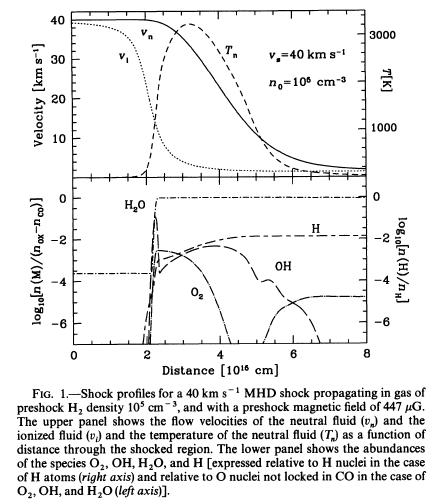
\includegraphics[width=13cm,height=!]{./E/Fig1_Kaufman_Neufeld.jpg}
    \end{center}
\end{minipage}
\begin{minipage}[t]{13cm}
%\vspace{-1cm}
  \begin{center}
    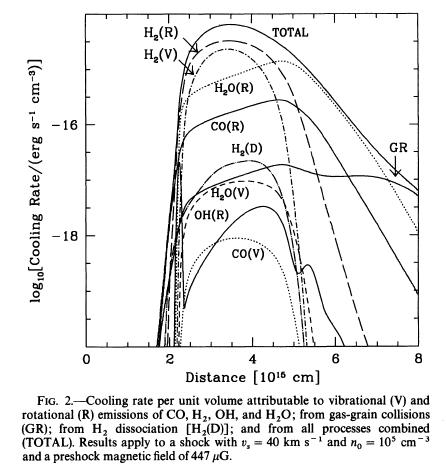
\includegraphics[width=13cm,height=!]{./E/Fig2_Kaufman_Neufeld.jpg}
    \end{center}
\end{minipage}


\foilhead{\textcolor{red}{E-\ref{item:Cshocks}} Structure of C shock:
  detailed calculations}

\begin{center}
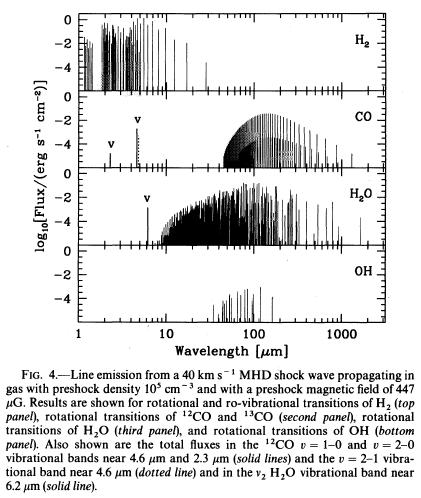
\includegraphics[width=14cm,height=!]{./E/Fig_4_Kaufman_Neufeld.jpg}
\end{center}

\leftheader{E-\ref{item:SNRs} SNRs}

\foilhead{\textcolor{red}{E-\ref{item:SNRs}}  Supernova Remnants}

References: 

\begin{itemize}

\item Lequeux, ``The interstellar medium'' (like Spitzer 1978).
\item Rohlfs \& Wilson ``Tools of Radioastronomy'' (emphasis on the
  synchrotron diagnostic). 
\item Tielens.
\end{itemize}

\foilhead{\textcolor{red}{E-\ref{item:SNRs}}  Supernova Remnants}


\begin{itemize}

\item There are three broad phases in the expansion of a SN shock
  wave:

\begin{enumerate}
\item a phase of free expansion, where the density of the ejected
  material is much larger than the density of the surrounding
  medium. This phase ends $\sim$60~yr after the SN event. It has been
  studied extensively in extragalactic SNe.

\item a phase of adiabatic expansion, where radiative losses are
  negligible, and where the temperature progressively cools through
  the work applied on the swept up ISM. 

\item an isothermal phase, where the remnant's energy is lost by
  radiation, and which ends when the SNR shell velocity is of order of
  the velocity dispersion in the ISM ($\sim$ the sound speed, or
  10~km~s$^{-1}$ in the diffuse ionised ISM at $10^4$~K).  

\end{enumerate}


\item SNRs of all types inject $\sim 10^{50}$~erg through a shocked
  shell driving into the ISM. SNe Ib/II may lead to {\em Plerions}:
 shell remnants filled with relativistic gas excited by a central
 pulsar. 

\end{itemize}


\foilhead{\textcolor{red}{E-\ref{item:SNRs}}  SNRs examples: Vela\footnote{G263.806$-$03.371}}


\begin{minipage}[t]{13cm}
%\vspace{-1cm}
  \begin{center}
IRAS~100$\mu$m.
    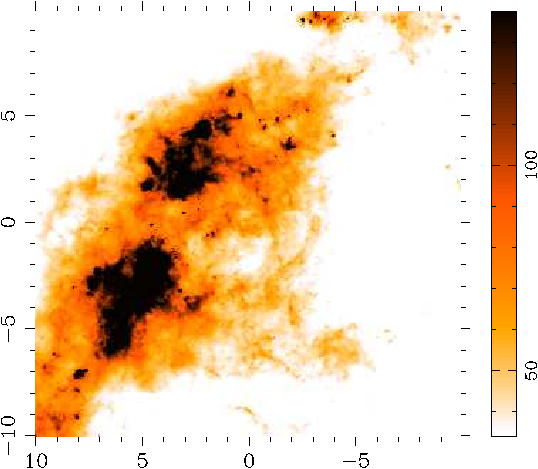
\includegraphics[width=12cm,height=!]{./E/VelaX_100um.pdf}
    \end{center}
\end{minipage}
\begin{minipage}[t]{13cm}
%\vspace{-1cm}
  \begin{center}
ROSAT broad band.
    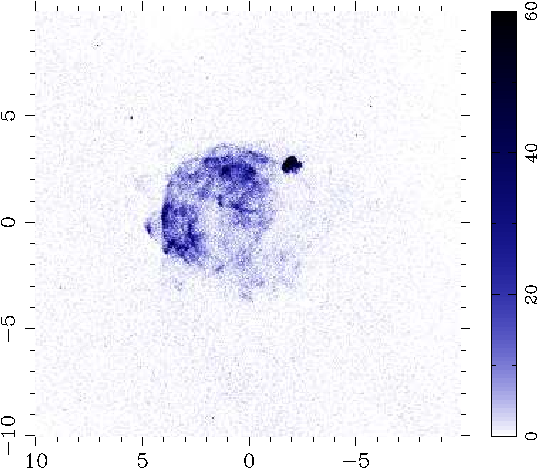
\includegraphics[width=12cm,height=!]{./E/VelaX_RASS_broad.pdf}
    \end{center}
\end{minipage}


\foilhead{\textcolor{red}{E-\ref{item:SNRs}} SNRs examples:
  Vela\footnote{Distance to Vela is $\sim$250~pc $\rightarrow$ 1~deg
    $\sim 5$~pc }}


\begin{minipage}[t]{10cm}
\vspace{-15cm}
{\small Hales et al. 2004, ApJ, 613, 977. \\
Bock et al., 1998, ApJ, 116, 1886.\\
Blondin et al. 2001, ApJ, 563, 806. }
  \begin{center}
    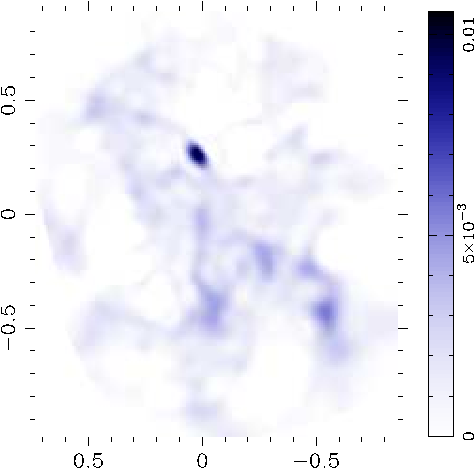
\includegraphics[width=10cm,height=!]{./E/vela_CBI.pdf}
    \end{center}
\end{minipage}
\begin{minipage}[t]{15cm}
%\vspace{-1cm}
%
 \begin{center}
    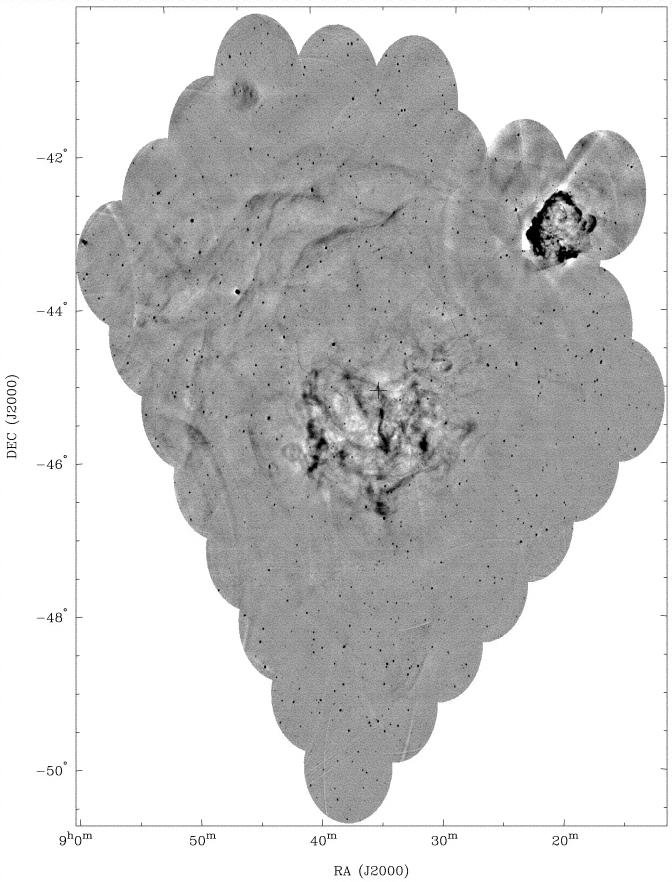
\includegraphics[width=12cm,height=!]{./E/vela_large_843MHz.jpg}
    \end{center}
\end{minipage}



\foilhead{\textcolor{red}{E-\ref{item:SNRs}}  SNRs examples: PWNe}


\begin{minipage}[t]{10cm}
%\vspace{-1cm}
  \begin{center}
    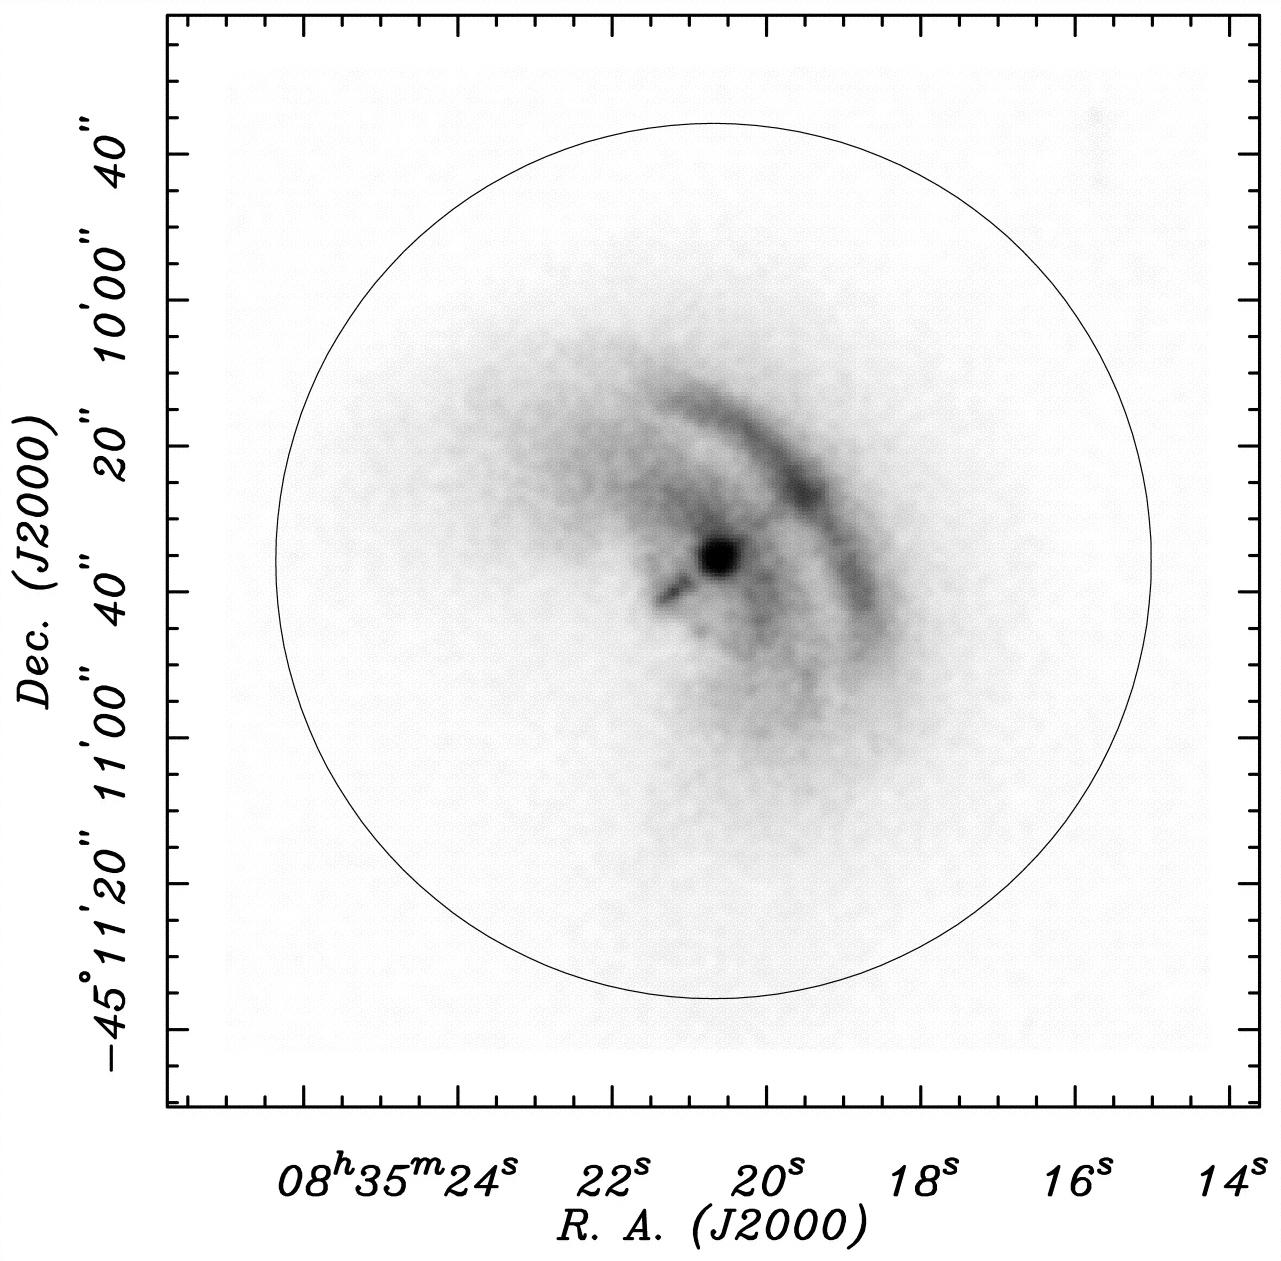
\includegraphics[width=10cm,height=!]{./E/fg3a_helfand.jpg}
    \end{center}
\end{minipage}
\begin{minipage}[t]{15cm}
%\vspace{-1cm}
  \begin{center}
    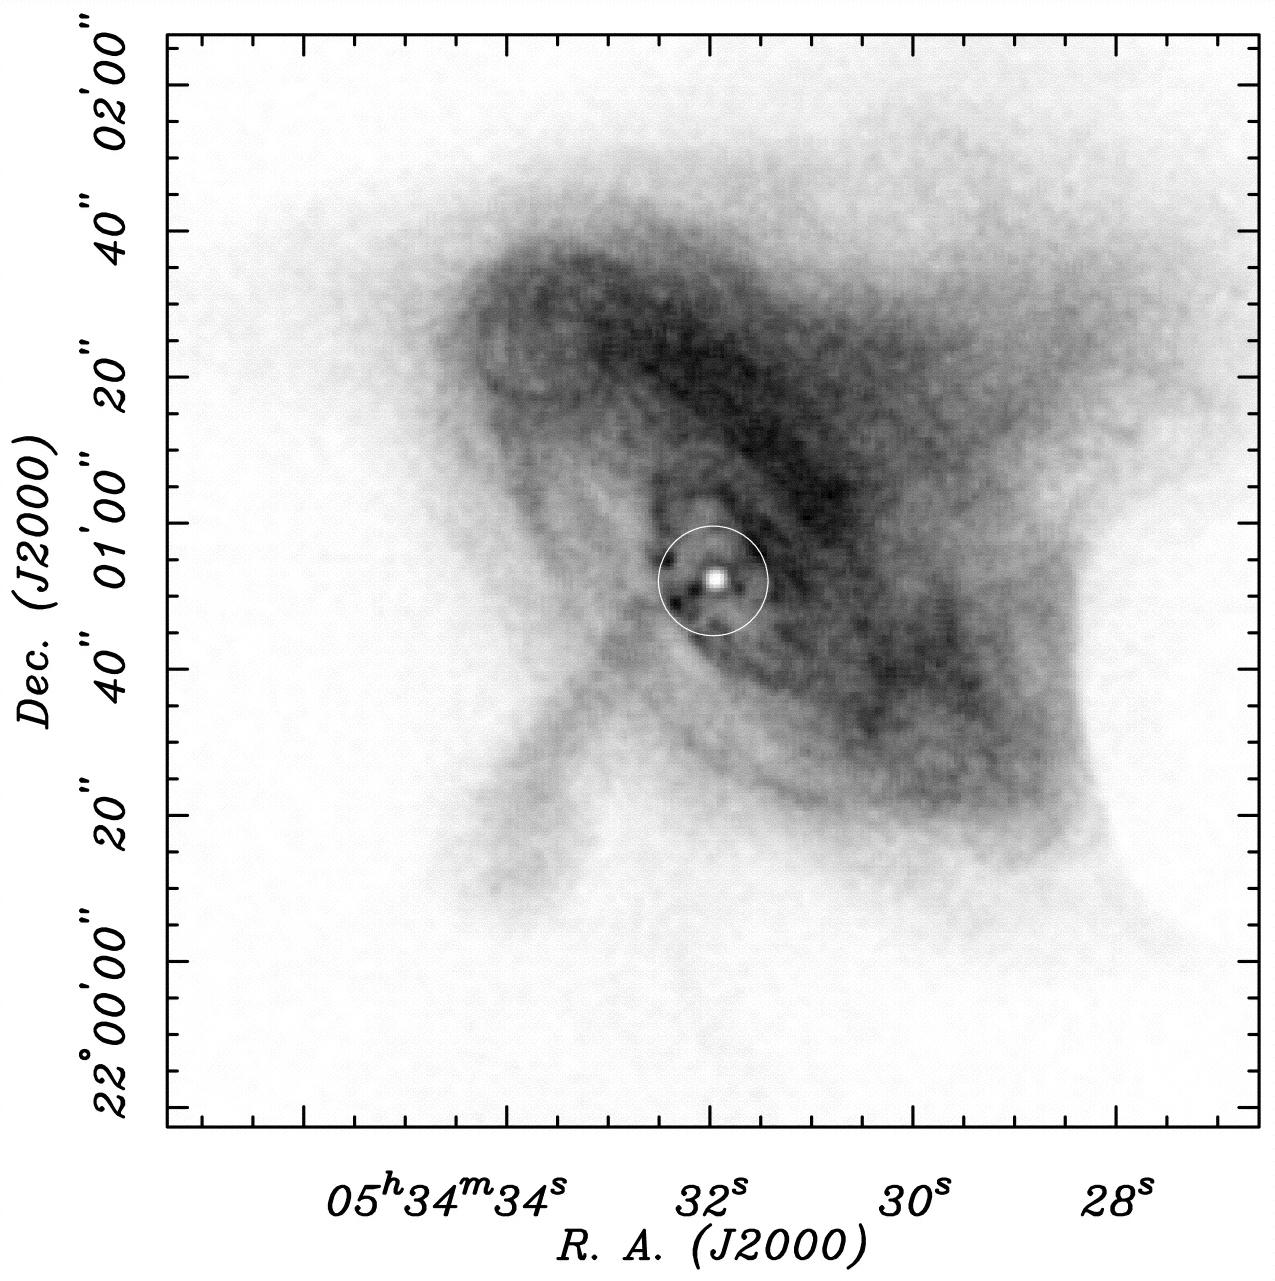
\includegraphics[width=10cm,height=!]{./E/fg3b_helfand.jpg}
    \end{center}
\end{minipage}

Helfand et al. 2001, ApJ, 556, 380. Note the age of both PWNe is very
different (Vela X is $\sim 10^4$~yr, see Blondin et al.). The circles
have equal radii of $\sim$0.05~pc. The Vela~X PSR radiates as a
$1.7~10^6$~K blackbody 10~km in radius, and the diffuse emission is
synchrotron. That the arcs are not complete rings may be due to the
head-light effect in the outflowing relativistic expansion.

\foilhead{\textcolor{red}{E-\ref{item:SNRs}}  SNR free-expansion
  phase}

\begin{itemize}

\item The SN event ejects the stellar envelope at $\sim
  10^4$~km~s$^{-1}$. 

\item For fully ionised gas the mean free path involves the Coulomb
  cross section of protons:
\begin{equation}
  l = m^2 v^4 / (Z^2 n\, e^4  \ln \Lambda ), ~\text{with} ~\Lambda =
1.3~10^4 T^{3/2} / n_e^{1/2}.  \label{eq:coulombfreepath}
\end{equation}

\item At $v\sim 10^4$~km~s$^{-1}$, the Coulomb cross section is so low
  that $l \sim 400$~pc for protons, so that they would escape the
  envelope. 

\item But a small magnetic field of only $\sim 1\mu$~G confines the
protons to Larmor radii of only $\sim 10^{-8}$~pc. Thus the
freely-expanding SNRs are MHD shocks.

\item The free-expansion phase ends when the SNR expansion has swept
  up enough mass to slow down due to momentum conversation. 

This occurs when when the mass swept by the envelope, $\frac{4}{3}\pi
r_s^3 \rho_0$, where $\rho_0$ is the surrounding density, is similar
to the mass of the ejecta, $M_\mathrm{ej}$. For $n_0 \approx
1~$cm$^{-3}$ and $M_\mathrm{ej} = 0.25~$M$_\odot$ (type Ia) we have
$r_s = 1.3~$pc, which is reached only 60~yr after the explosion if the
expansion velocity is 20000~km~s$^{-1}$.


\end{itemize}

\foilhead{\textcolor{red}{E-\ref{item:SNRs}} SNR adiabatic (Sedov)
  expansion phase}

\begin{itemize}

\item {\em Adiabatic} expansion means that the postshock temperature
  is so high that radiative losses are negligible. The mechanical
  SN energy $E$ is constant. 

\item Sedov (1959) showed that adiabatic expansion is self-similar:
  its macroscopic parameters are related by power-laws (see
  Chap.~A). In the Sedov phase, 
\begin{itemize}
\item the fraction of $E$ that is thermal is $K_1 E$, with $K_1 =
  0.72$, 
\item the ratio $K_2 = P_1 / \langle P \rangle = 2.13$, where
  $P_1$ is the pressure immediately behind the shock, and $\langle P
  \rangle$ is the average pressure inside the spherical remnant.

\end{itemize}
\end{itemize}

\foilhead{\textcolor{red}{E-\ref{item:SNRs}} SNR adiabatic (Sedov)
  expansion phase}

Once the expansion slows down to, say, 1000~km~s$^{-1}$, the magnetic
energy density is negligible compared to the thermal energy density
and we can use the J-shock results.

\begin{itemize}


\item With the above results from Sedov, and since for an ideal gas
  $\langle P \rangle = \frac{2}{3} K_1 E \frac{3}{4 \pi r_s^3}$, we
  have $ P_1 = K E / (2 \pi r_s^3)$, where $K = K_1 K_2$.

\item In the limit of a stron shock, $M \gg 1$, the Rankine-Hugoniot
  relations give $v_0 = \sqrt{ \frac{4  P_1}{3 \rho_0}}$, and since
  the shock velocity $v_s \approx v_0$, we obtain 
\begin{equation}
 v_s = \sqrt{ \frac{2 K E}{3 \pi r_s^3}} ~. \label{eq:adiavs}
\end{equation}


\end{itemize}

\foilhead{\textcolor{red}{E-\ref{item:SNRs}} SNR adiabatic (Sedov)
  expansion phase}


\begin{itemize}

\item Integrating Eq~\ref{eq:adiavs}, 
\begin{eqnarray}
r_s  &  =  &  \left( \frac{5}{2} \right)^{2/5} \left( \frac{2KE}{3\pi
  \rho_0}  \right)^{1/5} t^{2/5} , \nonumber \\ 
     &  =  & 0.26 ~ \left( \frac{n_H}{\mathrm{cm}^{-3}}
\right)^{1/5} \left( \frac{t}{\mathrm{yr}} \right) ^{2/5} \left(
\frac{E}{4~10^{50}~\mathrm{erg}} \right)^{1/5} ~~\mathrm{pc}.  \nonumber
\end{eqnarray}

\item again, with the strong shock conditions Eq.~\ref{eq:Jshock1} to  \ref{eq:Jshock2},
\begin{equation}
T_1 = \frac{3}{16k} \mu m_H v_s^2 = 1.5~10^{11}~\left(
\frac{n_H}{\mathrm{cm}^{-3}} \right)^{-2/5} \left(
  \frac{t}{\mathrm{yr}}  \right)^{-6/5} \left(
  \frac{E}{4~10^{50}~\mathrm{erg}} \right)^{1/5} ~\mathrm{K}.  \label{eq:Tshock}
\end{equation}
\item we see that the $T$ increases towards the centre, which reflects
  the neglect of radiative losses, and the fact that $v_s$ was higher
  when the central layers were overtaken by the shock.


\end{itemize}

\foilhead{\textcolor{red}{E-\ref{item:SNRs}} adiabatic expansion:
  thermal conductivity }

\begin{itemize}


\item However, in the absence of strong magnetic fields, the Coulomb
  mean free path $l$ (Eq.~\ref{eq:coulombfreepath}) is so high that
  diffusion is important, with thermal conductivity 

\begin{equation}
\kappa = \frac{5}{3} \frac{k T}{\langle v_{T} \rangle} l ~n
\frac{3k}{m}, ~~\text{with}~ \langle v_{T} \rangle = (3 k T /
m)^{1/2}. 
\end{equation}

\item Solving for the thermal balance including the heat flux $Q = -
  \kappa \nabla T$ leads to uniform temperatures in the SNR interior
  (Chevalier 1975, ApJ, 198, 355):

\begin{equation} T \approx
1.4~10^{10}~\left(\frac{n_0}{\mathrm{cm}^{-3}}\right)^{-1} \left(
\frac{r_s}{\mathrm{pc}} \right)^{-3} \frac{E}{10^{51}~erg} ~
\mathrm{K}. \label{eq:Tcond}
\end{equation}

\item However, a finite magnetic field exists inside the remnant, so
  that the mean free path and the conductivity $\kappa$ are reduced.
  The real temperature inside the remnant thus lies in between
  Eq.~\ref{eq:Tshock} and  Eq.~\ref{eq:Tcond}. 


\end{itemize}

\foilhead{\textcolor{red}{E-\ref{item:SNRs}} adiabatic expansion:
  reverse shock }

\begin{itemize}

\item An more accurate (numerical) treatment shows that the transition
  between free and adiabatic expansion generates a reverse shock.

\item The reverse shock propagates inwards, towards the centre of the
  ejected matter.

\item Qualitatively, the reverse shock stems from the pressure
  increment behind the shock front. The finite radiative losses lower
  the temperature inwards and away from the shock front. Thus the
  sound speed decreases inwards, and the pressure perturbation right
  behind the (outer) shock turns into an inner, or reverse, shock.

\item After the passage of the reverse shock the SNR expansion becomes
  truly adiabatic.
\end{itemize}

\foilhead{\textcolor{red}{E-\ref{item:SNRs}} Isothermal expansion }

\begin{itemize}
\item When the postshock temperature falls below $T_1 \approx 10^6$~K,
  metals start recombining, and radiative cooling is strongly enhanced
  through line emission from ions of C, N and O.

\item Energy is no longer conserved - rather, the expansion of the
  remnant is controled by momentum conversation.

\item The transition into the isothermal phase occurs at an age of
  $\sim 10^{4}$~yr, for an ambient density $n_0 \sim 1~$cm$^{-3}$, a
  shell radius $\sim 15$~pc, and an expansion velocity of
  85~km~s$^{-1}$. 
\end{itemize}


\foilhead{\textcolor{red}{E-\ref{item:SNRs}} Isothermal expansion }

\begin{itemize}
\item Momentum conservation requires that $M v_s$ is constant, where
  $M$ is the ISM mass swept-up by the remnant:
\[ \frac{4}{3} \pi r_s^3 \rho_0 v_s = \mathrm{constant}. \]

\item Integration then gives

\[ r_s = r_\mathrm{rad} \left( \frac{8 t }{5 t_\mathrm{rad}} -
\frac{3}{5} \right)^{1/4}, \] 

where $r_\mathrm{rad}$ and $t_\mathrm{rad}$ are the radius and age of
the remnant at the start of the isothermal phase. 

\end{itemize}

\foilhead{\textcolor{red}{E-\ref{item:SNRs}} Final mixing with the
  ISM}

\begin{itemize}

\item When the age of the remant is of order $10^6$~yr, its radius
  will be $\sim$40~pc, and $v_s \sim 10~$km~s$^{-1}$ - comparable to
  the sound speed of $10^4$~K `warm-ionised' ISM with $n_0 =
  1~$cm$^{-3}$. Thus the remnant will no longer be supersonic, and
  will mix with the ISM. 

\item The efficiency $\eta$ for the input of mechanical SN energy $E$
  into the ISM is 
\[ \eta = \frac{1}{2} M_f v_f^2  / E  , \]
where $M_f$ and $v_f$ are the final mass and velocity of the
remnant. Lequeux (2005) shows that $\eta \approx 0.03$.

\end{itemize}


\leftheader{E-\ref{item:HIIs} Ionization fronts}

\foilhead{\textcolor{red}{E-\ref{item:HIIs}} Dynamics of H\,{\sc ii}
  regions }

References: 

\begin{itemize}

\item Lequeux,  2005, ``The interstellar medium''.
\item Tenorio-Table \& Bodenheimer, 1988, ARA\&A, 26, 145
\item Kaplan \& Pikelner, 1970, ``The interstellar medium''.
\item Tielens, 2005. 
\end{itemize}


\foilhead{\textcolor{red}{E-\ref{item:HIIs}} Dynamics of H\,{\sc ii}
  regions }

Given an instantaneous proton density $n_p(t)$, ionisation equilibrium
applied to a whole H\,{\sc ii} region gives its size, the
Str\"omgren radius:
\begin{equation}
r_S = \left( \frac{3 \pi}{4}  \frac{S}{n_e n_p \alpha_2}
\right)^{1/3}, 
\end{equation}
where $S$ is the stellar-photon-luminosity in the Lyman continuum.

However the ionised gas is at a higher pressure than the
surroundings. If the proton density is uniform, in the ionised region
number densities are at least a factor of 2 higher than in neutral
gas, and temperatures are $\sim 10^4$~K against $\sim 10-100$~K in
the atomic/molecular gas. Thus H\,{\sc ii} regions are bound to
expand, and their densities will decrease. 

We will first quantify the dynamics of the ionisation front, and then
consider the pressure wave propagating in the neutral gas as a
precursor shock. 

\foilhead{\textcolor{red}{E-\ref{item:HIIs}} The ionisation front}

In plane-parallel geometry, the equations describing the inertia of
the front are:
\begin{eqnarray}
\rho_0 v_0  & = & \rho_1 v_1 , \text{~~mass continuity} \\
\rho_0 v_0^2 + P_0  &    =   & \rho_1 v_1^2 + P_1,  \text{~~ momentum equation}.
\end{eqnarray}
With 
\begin{eqnarray}
P_i &  =  &  \rho_i k T / (\mu_i m_H) , ~~\text{and}, ~\\
c_i  & = & \sqrt{\gamma k T /  (\mu_i m_H) } , ~~\text{ the sound
  speed}, 
\end{eqnarray}
we see that $P_i = c_i^2 \rho_i / \gamma$. 

\foilhead{\textcolor{red}{E-\ref{item:HIIs}} The ionisation front}

We can combine the above equations to give (\textcolor{red}{tarea})
\begin{equation}
\frac{\rho_1}{\rho_0} =  \frac{1}{2} \frac{c_0^2}{c_1^2} \left[
(M^2 + 1) \pm \sqrt{ (M^2+1)^2 - 4M^2 \frac{C_1^2}{C_0^2}} 
\right] , \label{eq:rhofrac}
\end{equation}
where $M = v_0 /c_0 $ is the Mach number of the ionisation front. 
The condition that the square root be real requires 
(\textcolor{red}{tarea})
\begin{equation}
M^2 - 2M \frac{c_1}{c_0} + 1 > 0, 
\end{equation}
so that the only possible values for $M$ are $ M < M_D$ or $ M > M_R$,
where 
\begin{eqnarray}
M_R  & =  & \frac{c_1}{c_0} \left( 1 + \sqrt{ 1 - \frac{c_0^2}{c_1^2} }
\right), \\
M_D  & =  & \frac{c_1}{c_0} \left( 1 - \sqrt{ 1 - \frac{c_0^2}{c_1^2} }
\right). 
\end{eqnarray}



\foilhead{\textcolor{red}{E-\ref{item:HIIs}} The ionisation front}

Since $T_0\ll T_1$, $c_0 \ll c_1$ and 
\begin{eqnarray}
M_R  & \approx  & 2 c_1/c_0, \\
M_D  & \approx  & c_0/ (2 c_1)
\end{eqnarray}

For either the `R' or `D' critical solutions, we have 
$M^2 + 1 = 2 M c_1/c_0$, so that Eq.~\ref{eq:rhofrac} gives 
\begin{equation}
\frac{\rho_1}{\rho_0}  = M \frac{c_0}{c_1} = \frac{v_0}{c_1}.
\end{equation}
The mass continuity equation then gives 
\begin{equation}
v_1 = \rho_0 v_0 / \rho_1 = c_1. 
\end{equation}

We see that for the critical values of $M$ the downstream velocity of
the gas is equal to the sound speed $c_1$.  We will now turn to a
detailed analysis of the critical solutions. 

%\end{equation} 
%\begin{eqnarray}
%\rho_0 v_0  & = & \rho_1 v_1 , \text{~~mass continuity} \\
%\rho_0 v_0^2 + P_0  &    =   & \rho_1 v_1^2 + P_1,  \text{~~ momentum equation}.
%\end{eqnarray}
%With 
%\begin{eqnarray}
%P_i &  =  &  \rho_i k T / (\mu_i m_H) , ~~\text{and}, ~\\
%c_i  & = & \sqrt{\gamma k T /  (\mu_i m_H) } , ~~\text{ the sound
%  speed}, 
%\end{eqnarray}
%we see that $P_i = c_i^2 \rho_i / \gamma$. 
%


\foilhead{\textcolor{red}{E-\ref{item:HIIs}} The ionisation front}

In plane-parallel geometry, the mass continuity equation gives

\begin{equation}
\rho_0 v_0 = \rho_1 v_1 = J,  \label{eq:massHII}
\end{equation}
where 
\begin{equation}
 J = \mu_0 m_H S \frac{e^{-\tau}}{4\pi r_s^2}
\end{equation}
is the flux of hydrogen atoms through the front, and $\tau = n_d
\sigma_d r_s$ is an average Lyman-continuum opacity mostly due to dust
inside the H\,{\sc ii} region (in the on-the-spot approximation the
contribution of opacity from residual atomic hydrogen is compensated
by recombinations).



\foilhead{\textcolor{red}{E-\ref{item:HIIs}} The ionisation front}

The momentum-conservation equation,
\begin{equation}
\rho_0 v_0^2 + P_0    =  \rho_1 v_1^2 + P_1, 
\end{equation}
can be written 
\begin{equation}
\rho_0 \left(\frac{k T_0}{\mu_0 m_H} + v_0^2 \right)  = 
\rho_1 \left(\frac{k T_1}{\mu_1 m_H} + v_1^2 \right),  \label{eq:momentumHII}
\end{equation}
where we have neglected radiation pressure (?` ojo?). 


\foilhead{\textcolor{red}{E-\ref{item:HIIs}} The ionisation front}

We will assume that the ionised gas behind the ionisation front
expands freely into the H\,{\sc ii} region, at a velocity close to the
sound speed (or close to the thermal rms speed) - this is exactly true
for the critical `R' or `D' solutions:
\[
v_1 \approx c_1 = \sqrt{ \frac{ \gamma k T_1  }{\mu_1 m_H}}.
\]
Substitution in the mass-continuity equation (Eq.~\ref{eq:massHII})
gives
\begin{eqnarray}
\rho_1 &  =  & J / c_1, \label{eq:dum1} \\
\rho_0  &  =  & J / v_0. \label{eq:dum2}
\end{eqnarray}


\foilhead{\textcolor{red}{E-\ref{item:HIIs}} The ionisation front}

With Eq.~\ref{eq:dum1} and \ref{eq:dum2}, and using momentum
conservation, Eq.~\ref{eq:momentumHII}, we obtain
(\textcolor{red}{tarea}) 
\begin{equation}
v_0 + \frac{1}{v_0} \frac{k T_0}{\mu_1 m_H} = (\gamma + 1) \sqrt{ \frac{k
  T_1}{\gamma \mu_1 m_H} },
\end{equation}
whose solution for $v_0$ is (\textcolor{red}{tarea}) 
\begin{equation}
v_0 = \sqrt{ \frac{ (\gamma + 1)^2 k T_1   }{ 4 \gamma \mu_1 m_H  }  }
\pm \sqrt{  \frac{ (\gamma + 1)^2 k T_1 }{ 4 \gamma \mu_1 m_H}  -
  \frac{ k T_0 }{\mu_0 m_H} }.
\end{equation}
Since $T_0 \ll T_1$, 
\begin{equation}
v_0 = \sqrt{ \frac{ (\gamma + 1)^2 k T_1   }{ 4 \gamma \mu_1 m_H  }  }
\left\{   1 \pm  \left[ 1 -  \frac{ 2 \gamma}{ (\gamma + 1)^2 }
    \frac{\mu_1}{\mu_0} \frac{T_0}{T_1}  \right] \right\}. \label{eq:v0}
\end{equation}


\foilhead{\textcolor{red}{E-\ref{item:HIIs}} The ionisation front}

We see that we have two broad families of solutions, corresponding to
each sign in Eq.~\ref{eq:v0}. 
\begin{itemize}
\item For the plus sign, the factor in curled brackets $\left\{
... \right\}$ can be approximated to 1 for $T_0 \ll T_1$, so that 
\[ 
\frac{\rho_1}{\rho_0} = \frac{v_1}{v_0} = \frac{\gamma + 1}{\gamma}, 
\] 
so that $\rho_1 > \rho_0$. This is called a {\em compression wave}, or
the R solution (R is for rarefied gas, since the fronts meets gas of
lower density). 

\item For the minus sign, we go to first order in $T_0/T_1$ and obtain 
(\textcolor{red}{tarea})
\[ 
\frac{\rho_1}{\rho_0} = \frac{v_1}{v_0} = \frac{1}{\gamma + 1}
\frac{\mu_1 T_0}{\mu_0 T_1},
\] 
so that $\rho_1 \ll \rho_0$. This is called a {\em rarefaction wave},
or the D solution (D is for dense gas, since the fronts meets gas of
higher density).
\end{itemize}

\foilhead{\textcolor{red}{E-\ref{item:HIIs}} The ionisation front}

In order to estimate the temperature in the ionised gas behind the
front, $T_1$, we use the conservation of energy (cf. Eq.~{eq:energy}),
\begin{equation}
\rho_0 v_0 \left[ \overbrace{\frac{ \gamma k T_0 } {(\gamma - 1) \mu_0
      m_H}}^{ (u_0 + P_0 ) / \rho_0  } +
  \frac{1}{2}v_0^2 \right]  =
 \rho_0 v_0 \left[ \frac{ \gamma k T_0 } {(\gamma - 1) \mu_0 m_H} +
  \frac{1}{2}v_0^2 \right]  - \epsilon_0 J,
\end{equation}
where $\epsilon_0$ is the mean energy per photoelectron
(instantaneously behind the front we neglect radiative cooling, which
is important for the subsequent mixing of the ionised gas). Using mass
and momentum conservation, Eq.~\ref{eq:massHII} and
\ref{eq:momentumHII}, we obtain
\begin{equation}
v_0^2 = \frac{\gamma + 1}{\gamma -1 } \frac{k T_1 }{\mu_1 m_H} - 
\frac{2 \gamma}{\gamma - 1} \frac{ k T_0}{\mu_0 m_H} -
\frac{\epsilon_0}{m_H}.  \label{eq:dum3}
\end{equation}
We can then obtain $T_1$ given $T_0$ by equating Eq.~\ref{eq:v0} and
\ref{eq:dum3}. 

\foilhead{\textcolor{red}{E-\ref{item:HIIs}} The ionisation front}

In summary,
\begin{itemize}
\item D-critical fronts, $\rho_0 > \rho_1$.  \medskip
\begin{equation}\label{eq:D}
\begin{array}{rclcrcl}
T_1 &  =  &  \frac{\gamma-1 }{\gamma (\gamma + 1) } \frac{\mu_1
  \epsilon_0}{k},  &   ~~~  &  v_0  & = &  \frac{\mu_1 T_0}{\mu_0 T_1} \sqrt{
  \frac{ (\gamma - 1) \epsilon_0 }{ (\gamma  + 1)^3 m_H}
},  \vspace{1cm} \\ 
\frac{\rho_1}{\rho_0} &  = &  \frac{1}{\gamma + 1} \frac{\mu_1 T_0}{\mu_0
  T_1},  & ~~~  & \rho_0 &  = &  J \sqrt{  \frac{ (\gamma+1)^3}{\gamma
    - 1} \frac{m_H^3}{\epsilon_0}}. 
\end{array}
\end{equation}
With $\gamma = 5/3$\footnote{remember we are neglecting internal
  degrees of freedom, even for H$_2$}, we obtain $v_0 \approx
0.2~$km~s$^{-1}$, $\rho_1 / \rho_0 \approx 1/100$, and if $T_0 \sim
1000~$K then $T_1 \sim 3000--6000~$K. Further downstream the gas will
heat to its equilibrium value of $10^4$~K. Note that $\rho_0$ is
fixed.
\end{itemize}

\foilhead{\textcolor{red}{E-\ref{item:HIIs}} The ionisation front}
\begin{itemize}
\item R-critical fronts, $\rho_0 < \rho_1$.
\begin{equation} \label{eq:R}
\begin{array}{rclcrcl}
T_1 &  =  &  \frac{ \gamma( \gamma-1) }{ (\gamma + 1) } \frac{\mu_1
  \epsilon_0}{k},  &   ~~~  &  v_0  & = & \sqrt{
  \frac{ (\gamma^2 - 1) \epsilon_0 }{  m_H}
},  \vspace{1cm} \\ 
\frac{\rho_1}{\rho_0} &  = &  \frac{\gamma+1}{\gamma},  & ~~~  &
\rho_0 &  = &  J \sqrt{  \frac{ m_H^3}{ (\gamma^2 -1)\epsilon_0}}. 
\end{array}
\end{equation}
We have $\rho_1 / \rho_0 = 8/3$ and $v_0 \sim 26~$km~s$^{-1}$, so that
the front is supersonic. Note that 
\[
v_0 = \sqrt{\frac{ (\gamma^2 - 1) \epsilon_0 }{m_H}} = \rho_1 v_1  /
\rho_0 = \rho_1 c_1 / \rho_0 = 8/3 c_1, 
\]
the R front propagates at 8/3 ($\sim$ twice) the downstream sound speed.

\end{itemize}



\foilhead{\textcolor{red}{E-\ref{item:HIIs}} The precursor shock}


\begin{itemize}


\item We see from both Eq.~\ref{eq:D} and \ref{eq:R} that the
  upstream density $\rho_0$ is fixed by the ionising photon flux $J$
  and by $\epsilon_0$, both of which are functions of the central star
  spectrum. 

\item $\rho_0$ is in general different from $\rho_\mathrm{ISM}$, the
  ambient density in which the shock progresses. The front is
  therefore preceded by a density (i.e. pressure) perturbation, which
  travels at the sound speed set by $T_0$.

\item R-fronts are supersonic, so the precursor perturbation cannot
  travel away from the front.

\item D-fronts are subsonic ($\sim$ 0.2~km~s$^{-1}$), so the precursor
  perturbation can form a wave. Since $\rho_0$ is fixed by $J$, close
  to the central star (or early in the evolution of the H\,{\sc ii}
  region), $\rho_0 > \rho_\mathrm{ISM}$. 

\item In D-fronts the precursor wave will form a shock since the
  upstream gas is heated by the compression, so that $T_0 >
  T_\mathrm{ISM}$.  An approximate quantitative descriptions of the
  shock can be found in Spitzer (1978)

\end{itemize}



\foilhead{\textcolor{red}{E-\ref{item:HIIs}} Evolution of H\,{\sc ii}
  regions} 

\begin{itemize}

\item Turn-on phase.  \\

 An O star is suddenly turned-on in an infite and homogeneous medium,
 with a constant ionising photon luminosity $S$. Initially, for times
 short compared to the recombination timescale $\tau_\mathrm{rec} =
 (n_\mathrm{ISM} \alpha_2)^{-1} \approx 100~$yr for $n_\mathrm{ISM} =
 10^3$cm$^{-3}$, all photons from the star lead to ionisation, and the
 star ionises a sphere of radius $r(t)$, such that
\[ 
S t = \frac{4 \pi}{3} n_\mathrm{ISM} r^3(t).
\]
This sphere expands at a velocity 
\[
\frac{dr}{dt} = \frac{1}{3} \left( \frac{3 S}{4 \pi n_\mathrm{ISM}}  \right)^{1/3}  t^{-2/3},
\]
which at 100~yr is $\sim$4~10$^{3}$~km~s$^{-1}$.  {\bf this phase has
  never been observed, and the present description is
  unrealistic}. This phase is an R-front since the ionised gas is
hotter and denser (factor of 2). 

\end{itemize}



\foilhead{\textcolor{red}{E-\ref{item:HIIs}} Evolution of H\,{\sc ii}
  regions} 

\begin{itemize}

\item Approach to the Str\"omgren radius.  \\ 

Following the turn-on phase, at timescales of order
$\tau_\mathrm{rec}$ we must take into account recombination so that
the radius of the R-front is given by
\[
\frac{dr}{dt}  = \frac{1}{4 \pi r^2 n_\mathrm{ISM} } \left[ S -
  \frac{4}{3} \pi r^3 n_\mathrm{ISM}^2 \alpha_2    \right],
\]
where we have used the on-the-spot approx.
The solution to this equation is 
\[ 
r^3 = R_S^3 [ 1 - \exp( - n_\mathrm{ISM} \alpha_2 t) ],
\]
where $R_S$ is the Str\"omgren radius. 

Thus the front velocity will progressively decrease until it reaches
the `R'-critical value, after which it will jump down to the
`D'-critical value (somewhere close to the Str\"omgren radius). 

\end{itemize}



